\documentclass[11pt]{article}
\usepackage{fancyhdr}
\usepackage{tocloft}
\usepackage{graphicx}
\usepackage{calc}
\usepackage{amssymb}
\usepackage{color}
\usepackage[sc]{mathpazo}
\usepackage{url}
\usepackage{ifpdf}
\usepackage{bbding}
\usepackage{caption}
\usepackage{framed}
\usepackage{xcolor}
\usepackage{float}
\usepackage{wrapfig}
\usepackage{sidecap}
\linespread{1.0}
\oddsidemargin=0pt
\evensidemargin=0pt
\textwidth=6.5in
\topmargin=0pt
\headheight=0pt
\headsep=0pt
\textheight=9in
\setlength{\parindent}{0.25cm}
\newcommand\secfont{\fontfamily{cmss}\selectfont}%\textwidth 5.5truein
\newcommand\pifheading[1]{\noindent{\secfont\textbf{#1}:}}
\newcommand\yr{2016}
\def\lo{
\mathrel{\raise.3ex\hbox{$<$}\mkern-14mu\lower0.6ex\hbox{$\sim$}}
}
\def\hi{
\mathrel{\raise.3ex\hbox{$>$}\mkern-14mu\lower0.6ex\hbox{$\sim$}}
}

\textwidth = 6.5 in
\textheight = 9 in
\oddsidemargin = -0.00 in
\evensidemargin = +0.05 in
\topmargin = 0 in
\headheight = 0.0 in
\headsep = 0.0 in
\parskip = 0.05in

\newcommand\registered{{\ooalign{\hfil\raise .00ex\hbox{\scriptsize R}\hfil\crcr\mathhexbox20D}}}

%% Define a new 'leo' style for the package that will use a smaller font.
\makeatletter
\def\url@leostyle{%
  \@ifundefined{selectfont}{\def\UrlFont{\sf}}{\def\UrlFont{\small\ttfamily}}}
\makeatother
%% Now actually use the newly defined style.
\urlstyle{leostyle}
\newcommand\checkme[1]{\textcolor{blue}{\textbf{#1}}}
\newcounter{hours}\newcounter{minutes}
\newcommand\printtime{\setcounter{hours}{\time/60}\setcounter{minutes}{\time - \value{hours}*60}\thehours :\theminutes}
\newenvironment{packed_item}{
\begin{itemize}
 \setlength{\itemsep}{1pt}
 \setlength{\parskip}{0pt}
 \setlength{\parsep}{0pt}
}{\end{itemize}}

\newenvironment{packed_enum}{
\begin{enumerate}
 \setlength{\itemsep}{1pt}
 \setlength{\parskip}{0pt}
 \setlength{\parsep}{0pt}
}{\end{enumerate}}

\newenvironment{box_list}{
\begin{itemize}
 \setlength{\itemsep}{3pt}
 \setlength{\parskip}{0pt}
 \setlength{\parsep}{0pt}
}{\end{itemize}}

\newenvironment{packed_list}{
\begin{list}{\labelitemi}{\leftmargin=1em}
 \setlength{\itemsep}{3pt}
 \setlength{\parskip}{0pt}
 \setlength{\parsep}{0pt}
}{\end{list}}

\renewenvironment{quote}{%
  \list{}{%
    \leftmargin10pt   % this is the adjusting screw
    \rightmargin\leftmargin
  }
  \item\relax
}
{\endlist}

% definition of a new float type (refer to the caption package documentation)
\DeclareCaptionType{boxcaption}[Box]
\captionsetup[boxcaption]{position=top,labelfont=bf}

% definition of a shaded-like environment (see framed.sty)
\newenvironment{shadedframe}
  {\def\FrameCommand{\setlength\fboxsep{10pt}\fcolorbox{black}{shadecolor}}%
    \MakeFramed {\advance\hsize-\width \FrameRestore}}%
{\endMakeFramed}

\newenvironment{shadedbox}{%
  \def\FrameCommand{\colorbox{shadecolor}}%
  \MakeFramed {\FrameRestore}}%
 {\endMakeFramed}

% main environment
% syntax: \begin{myenv}{placement-specifiers}{color}{width}...\end{myenv}
\newenvironment{boxenv}[3]
  {\colorlet{shadecolor}{#2}%
    \begin{boxcaption}[#1]%
    \noindent\begin{minipage}{#3}
      \begin{shadedframe}
      }
  {\end{shadedframe}\end{minipage}\end{boxcaption}}

 % TOC
\usepackage{enumerate}
\begin{document}


\begin{figure}
  
\includegraphics[width=\linewidth/3]{title}
  \label{fig:title}
\end{figure}


\title{Lab Report 6: The Bipolar Junction Transistor (BJT)}


\author{Yuezhe Yao}

%\institute{Syracuse University}



\maketitle

\begin{abstract}
In Activity 1, we utilized a VI from a previous activity to 
measure, store and analyze the characteristic curves of a commercial BJT in a standard configuration known as the common-emitter configuration. In Activity 2, using these characteristic curves, we then designed, built and operated an important circuit known as the common-emitter amplifier. In Activity 3, we built a circuit known as the emitter follower. Finally in Activity 4, we investigated switching behavior of a transistor and use it to build a two-transistor logic gate.            
\end{abstract}

\medskip

\begingroup
\let\clearpage\relax
\tableofcontents
\endgroup

\medskip
\medskip


\section{Activity I - Measuring the Characteristic Curves of the MPS3904 Silicon npn Transistor in Common Emitter Configuration}

\begin{figure}[H]
 \begin{center}
  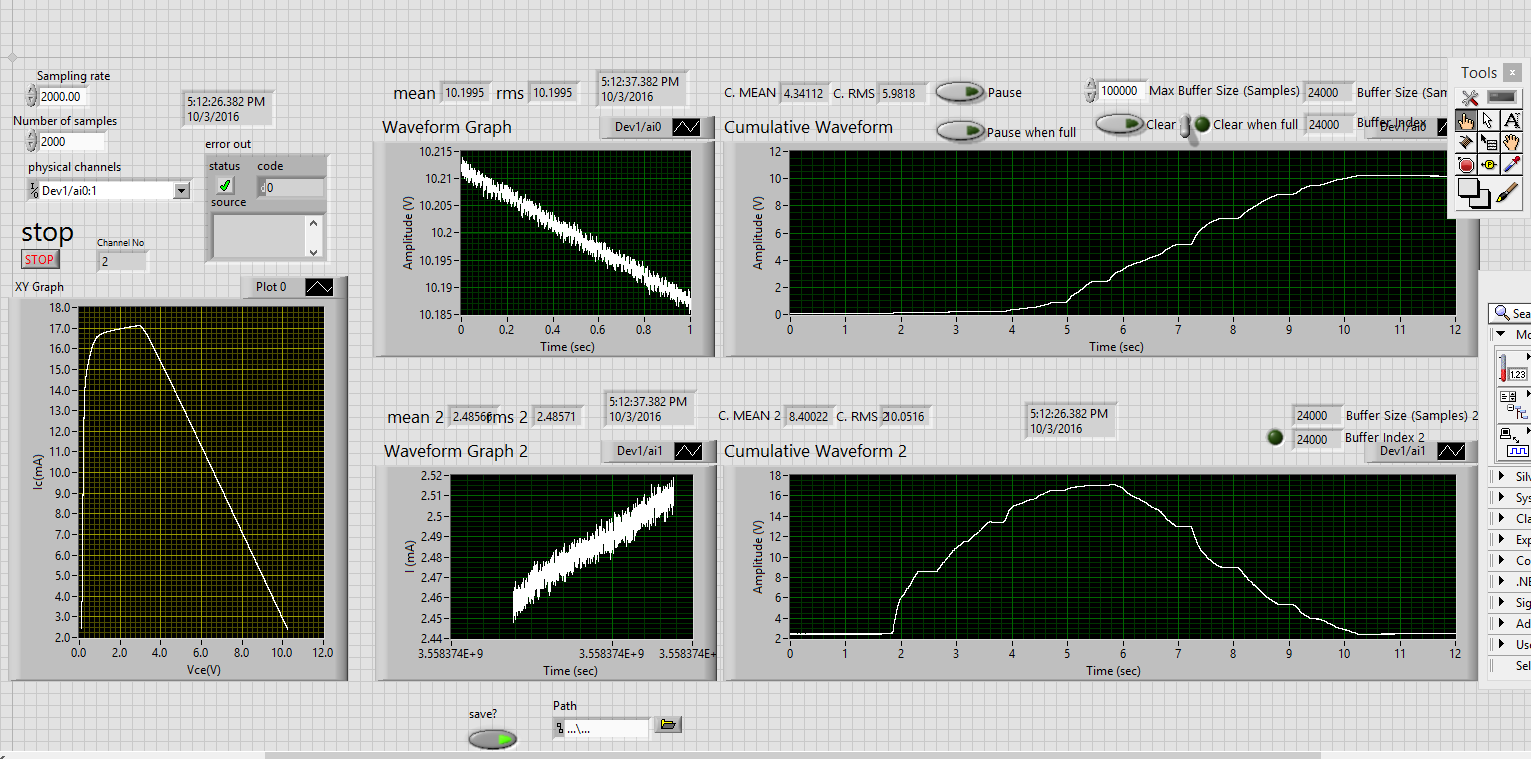
\includegraphics[width=\linewidth/1]{act1IB100}
  \caption{The front panel of the VI with $I_{\mathrm{B}}=100\mu A$.}
  \label{fig:act1IB100}
 \end{center}
\end{figure}

\begin{figure}[H]
 \begin{center}
  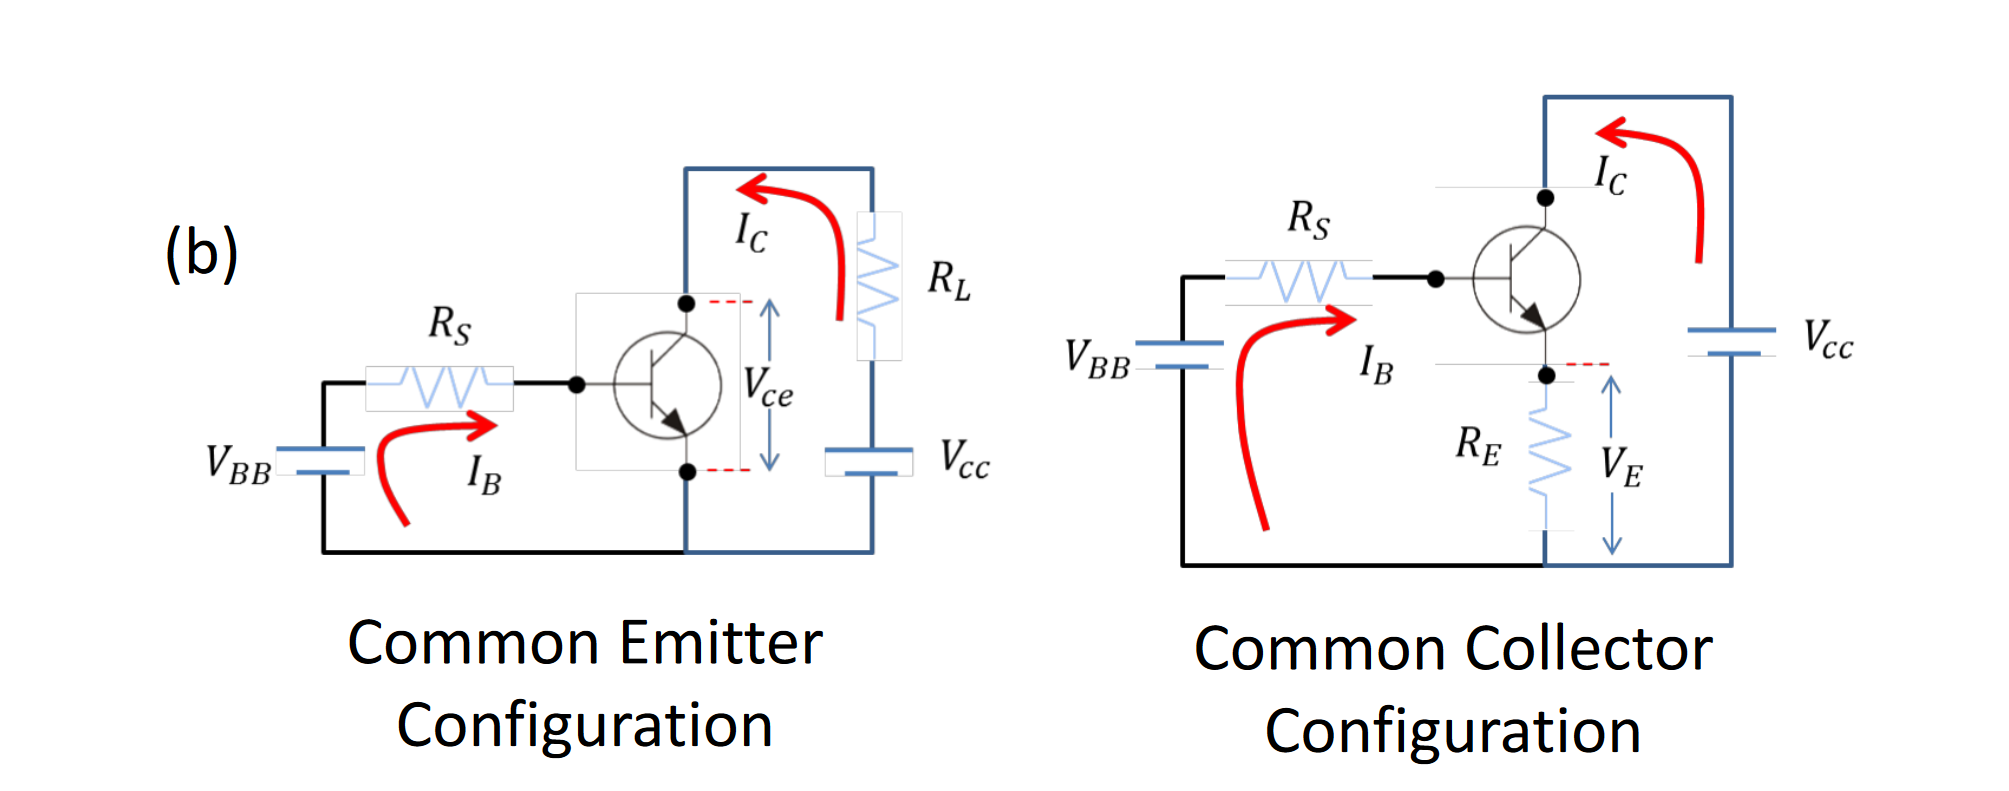
\includegraphics[width=\linewidth/1]{emitter}
  \caption{(b) Circuit schematics of 
transistor connections for CE and CC configurations. For
CC mode, the output is taken across $R_{\mathrm{E}}$.}
  \label{fig:emitter}
 \end{center}
\end{figure}

And we choose $R_{\mathrm{s}}=10k\Omega$ and $R_{\mathrm{L}}=470\Omega$, because $R_{\mathrm{s}}>>R_{\mathrm{in}} \approx \beta r_{\mathrm{e}}$. And at first we chose $R_{\mathrm{L}}=1k\Omega$, but then we found choosing $R_{\mathrm{s}}=470\Omega$ works better, so that voltage drop is readily measurable but not so large that at modest $I_{\mathrm{B}}$ the collector voltage drops too close to zero and the base-collector junction becomes forward biased.



\begin{figure}[H]
 \begin{center}
  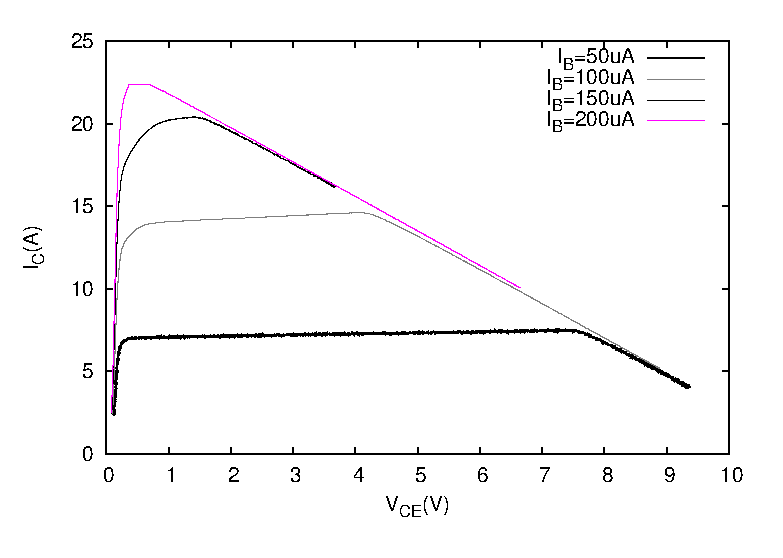
\includegraphics[width=\linewidth/1]{IcVce}
  \caption{The plot of $I_{\mathrm{c}}$ vs $V_{\mathrm{out}}$.}
  \label{fig:IcVce}
 \end{center}
\end{figure}

When we tried $I_{\mathrm{B}}=300 \mu A \ or \ 400 \mu A$, the current saturated, so we chose $I_{\mathrm{B}}=50 \mu A \ and \ 150 \mu A$ instead.



\section{Activity II - Designing and Building a Common-Emitter Amplifier}


\begin{figure}[H]
 \begin{center}
  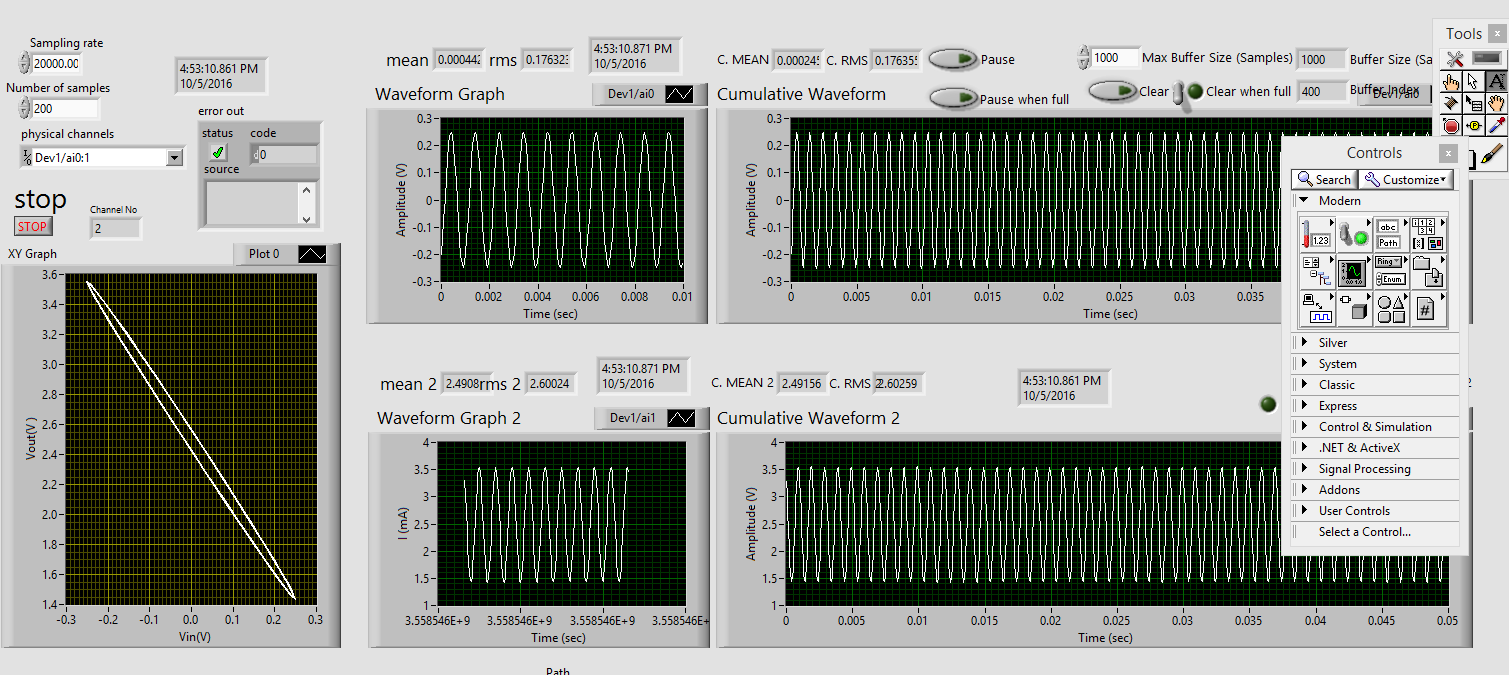
\includegraphics[width=\linewidth/1]{act2}
  \caption{The the front panel of the oscilloscope VI.}
  \label{fig:act2}
 \end{center}
\end{figure}

\begin{figure}[H]
 \begin{center}
  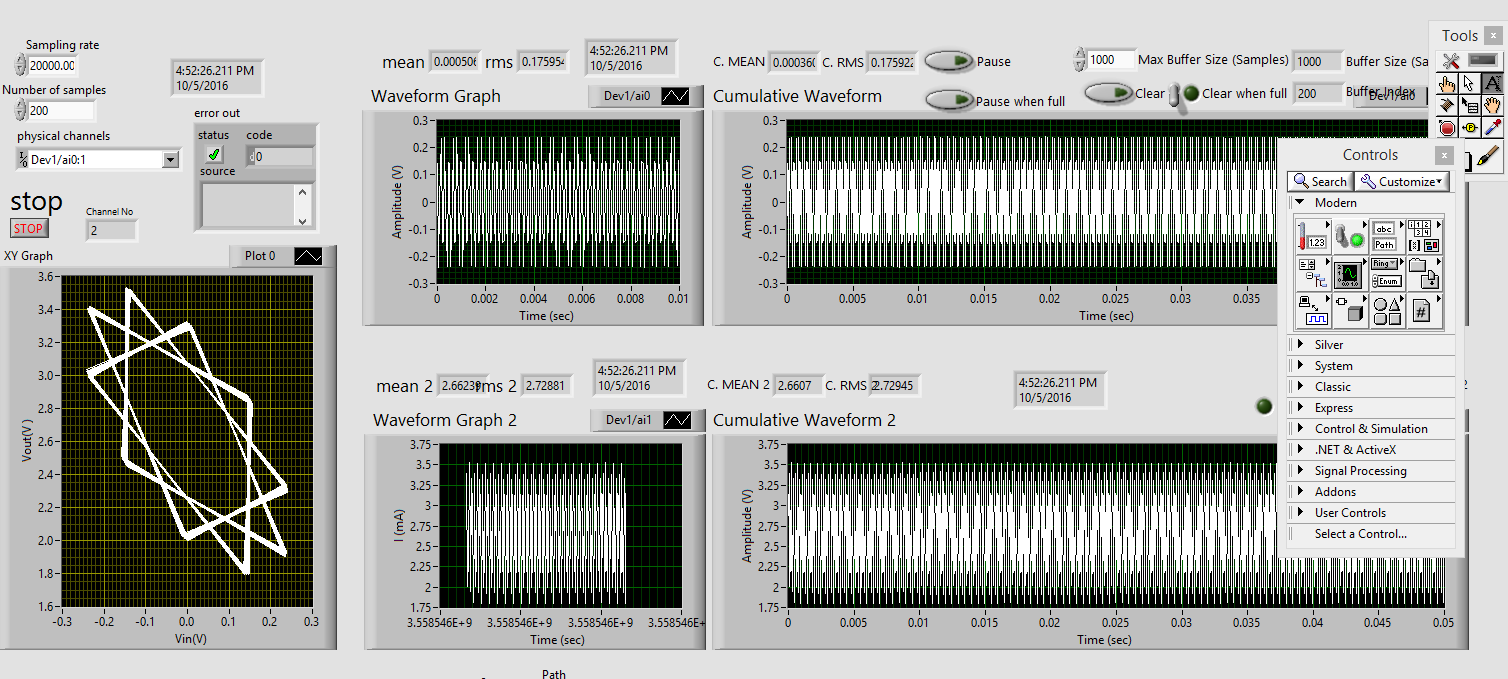
\includegraphics[width=\linewidth/1]{act2phaseshift}
  \caption{The the front panel of the oscilloscope VI (phase shift).}
  \label{fig:act2phaseshift}
 \end{center}
\end{figure}

\begin{figure}[H]
 \begin{center}
  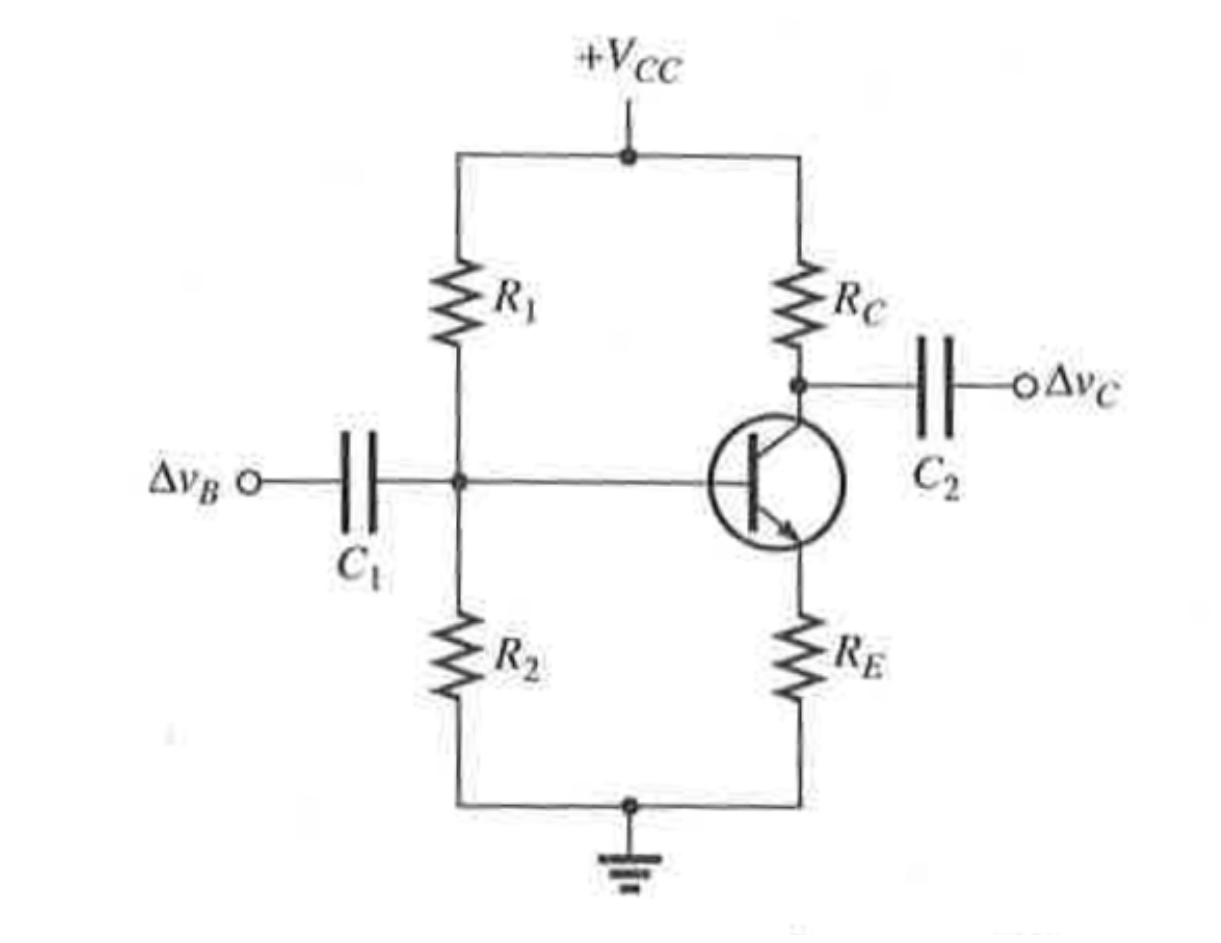
\includegraphics[width=\linewidth/1]{act2figure}
  \caption{Activity 2.}
  \label{fig:act2figure}
 \end{center}
\end{figure}

We chose $R_{\mathrm{1}}=100k \Omega$, $R_{\mathrm{2}}=20k \Omega$, $R_{\mathrm{c}}=4.7k \Omega$ and $R_{\mathrm{E}}=1k \Omega$. Because the voltage gain=5V, the output impedance $Z_{\mathrm{out}}=R_{\mathrm{E}}=1k \Omega$, so the $R_{\mathrm{c}}=R_{\mathrm{E}}*Voltage \ gain=1k*5=5k \Omega$. And because $R_{\mathrm{2}}<<R_{\mathrm{E}}*current \ gain=1k*100=100k \Omega$, so $R_{\mathrm{2}}=20k \Omega$ is fine. And for $R_{\mathrm{1}}$ and $R_{\mathrm{2}}$, their parallel resistance is less than the input impedance of the transistor.

$V_{\mathrm{supply}}=V_{\mathrm{CC}}=18V$. \\

From the image, we can see that the $V_{\mathrm{out}}$ difference is about 2.2V, and the $V_{\mathrm{in}}$ difference is about 0.5V, so it amplify about 2.2/0.5=4.4 times, which is consistent with the Voltage gain = 5. And there is also a phase shift, and if we change the input frequency a little bit, we can see some beautiful shapes like a star in the image because of the phase shift. In addition, the reason why the plot goes down is because, when we increase $V_{\mathrm{B}}$, $I_{\mathrm{B}}$ also increased, and so $V_{\mathrm{Rc}}$ increased, so the $V_{\mathrm{c}}$ difference  $\triangle V_{\mathrm{c}}$ decreased. The range of the input signal voltage is $0.6V<V_{\mathrm{in}}<{V_{\mathrm{supply}} \over {1+gain}}+0.6V$, if we choose $V_{\mathrm{supply}}=18V$, then the range is $0.6V<V_{\mathrm{in}}<{V_{\mathrm{supply}} \over {1+gain}}+0.6V=18/6+0.6=3.6V$.


\section{Activity III - Impedance Engineering with the Common-Collector (a.k.a. the Emitter Follower)}

\begin{figure}[H]
 \begin{center}
  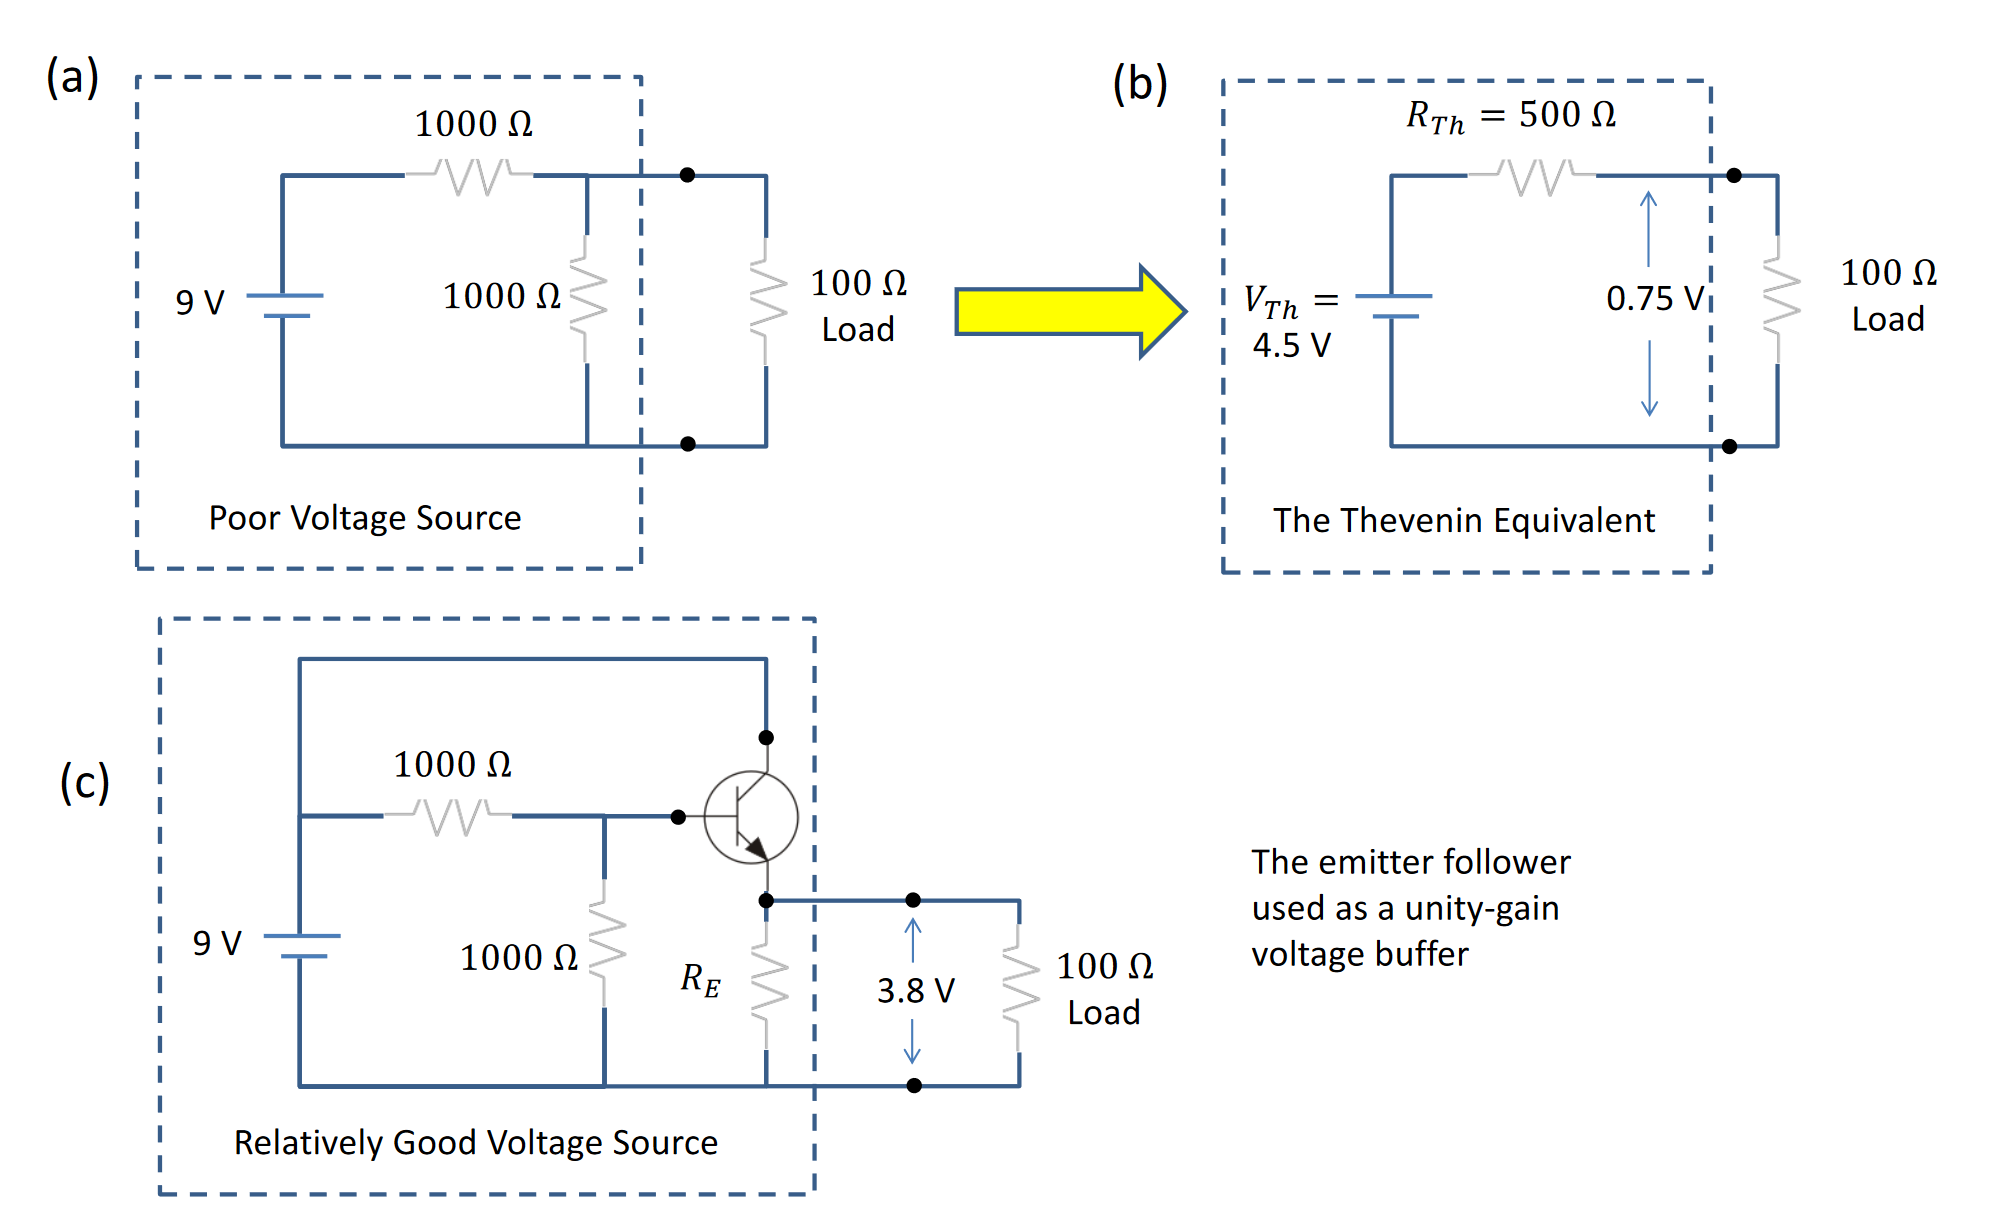
\includegraphics[width=\linewidth/1]{act3figure}
  \caption{Activity 3.}
  \label{fig:act3figure}
 \end{center}
\end{figure}

For the circuit in Activity 3(a), when the $100 \Omega$ resistor is removed, the voltage is 4.51V, which make sense because 9V/2=4.5V. When the voltage decrease to 1/2 the open circuit voltage, which is 2.25V, the resistance is $498 \Omega$, which is consistent with what we expect($500 \Omega$). And this value of the resistance is the output resistance of our voltage divider circuit, because:

Now let's say the output resistance of the voltage divider circuit is r, and the variable resistor we added is R, so the current I:

$I={V \over {r+R}}$

and also $I={V \over {2R}}$

$\Rightarrow r=R$

And for the circuit in Activity 3(c), when $I_{\mathrm{c}} \approx 10 \ mA$, we found $R_{\mathrm{E}} =362 \Omega $, so we chose $R_{\mathrm{E}} =348 \Omega $ in our circuit. Then we got the output voltage as 3.74V, which is close to 3.8V. When we replace the $100 \Omega$ resistor with a variable resistor and decrease the voltage to around 1.8-1.9V, we found the output impedance is $13.7 \Omega$.

In Fig.7 Act3a, because the $100 \Omega$ load is less than the output resistance which is $500 \Omega$, so you can't supply a voltage that is larger than 4.5/2=2.25V on that resistor, you can only get ${4.5 \over 6}=0.75V$. But for Fig.7 Act3c, because of the transistor, 4.5V-0.6V=3.9V, and 3.8V < 3.9V, so by choosing an appropriate $R_{\mathrm{E}}$ we can supply 3.8V across the $100 \Omega$ load.

\section{Activity IV - The BJT Switch and a Transistor-Transistor NOR Gate}

\begin{figure}[H]
 \begin{center}
  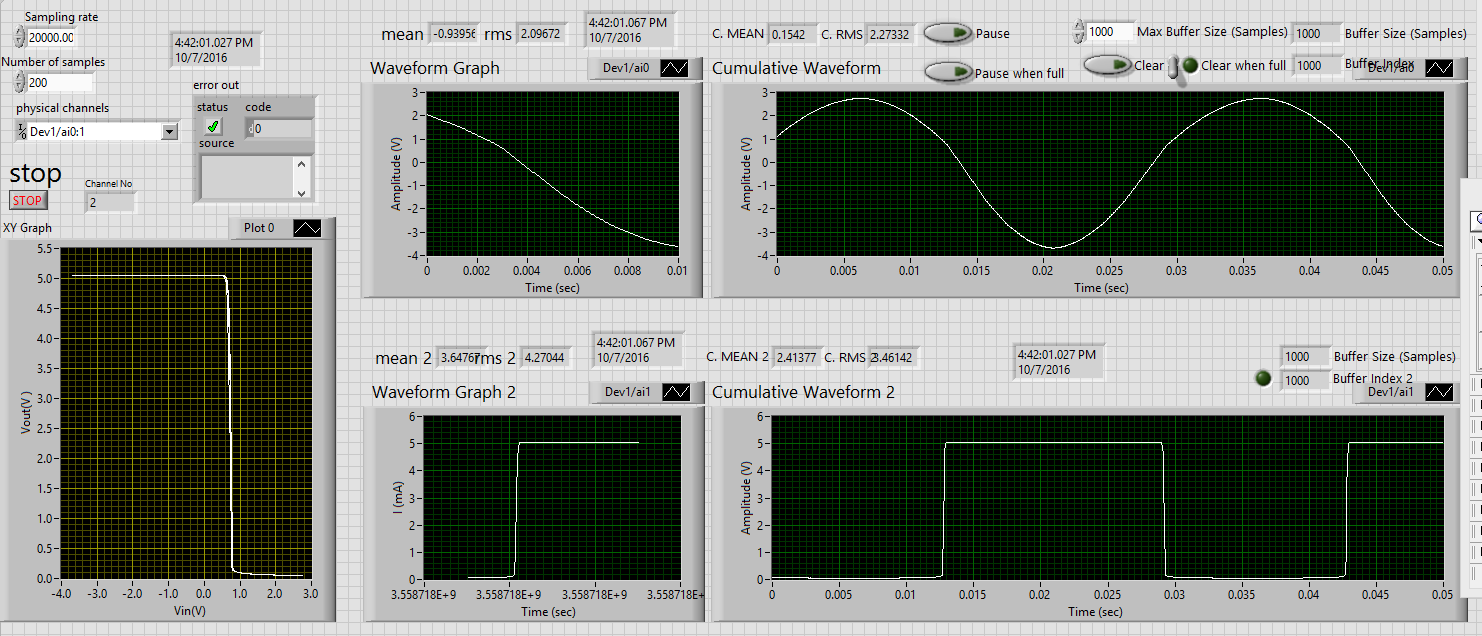
\includegraphics[width=\linewidth/1]{act4}
  \caption{The front panel of the BJT Switch.}
  \label{fig:act4}
 \end{center}
\end{figure}

From the image we can see that, the cut-off $V_{\mathrm{in}}$ is 0.6V, so when $V_{\mathrm{in}}<0.6V$, $V_{\mathrm{out}}=5V=V_{\mathrm{supply}}$ and $I_{\mathrm{c}}=0$, the base-emitter junction is reversed biased. And the saturation $V_{\mathrm{in}}$ is 0.8V, so when $V_{\mathrm{in}}>0.8V$, $V_{\mathrm{out}}$ drops towards zero, the BC junction becomes fully forward biased, and $I_{\mathrm{c}}$ is no longer a function of $I_{\mathrm{B}}$. 

And Fig.10 shows the The plot of $I_{\mathrm{c}}$ vs $V_{\mathrm{out}}$ with the load line ($V_{\mathrm{CC}}=5V$), we can see that the intersection of the load line and the plot shows what for $I_{\mathrm{B}} \geq 50 \mu A$, the transistor 
saturates and $V_{\mathrm{out}} \approx 0V$. On the other hand, if $I_{\mathrm{B}} \approx 0 \mu A$, then $V_{\mathrm{out}} \approx 5V$, and the transistor is cut-off.

And we also managed to make the NOR gate and construct the truth table that we expect successfully. In our circuit, if $V_{\mathrm{A}}$ or $V_{\mathrm{B}}$ is larger than 0.8V, we call a "1", and if it is smaller than 0.5V, we call a "0". So in Fig.9 below we can see that only when both $V_{\mathrm{A}}$ and $V_{\mathrm{B}}$ are smaller than 0.5V, the $V_{\mathrm{out}}$ is 5V, otherwise, $V_{\mathrm{out}}$ is 0V. So we call "1" for $V_{\mathrm{out}}=5V$, and "0" for $V_{\mathrm{out}}=0V$. In this way, we built a NOR gate.

\begin{figure}[H]
 \begin{center}
  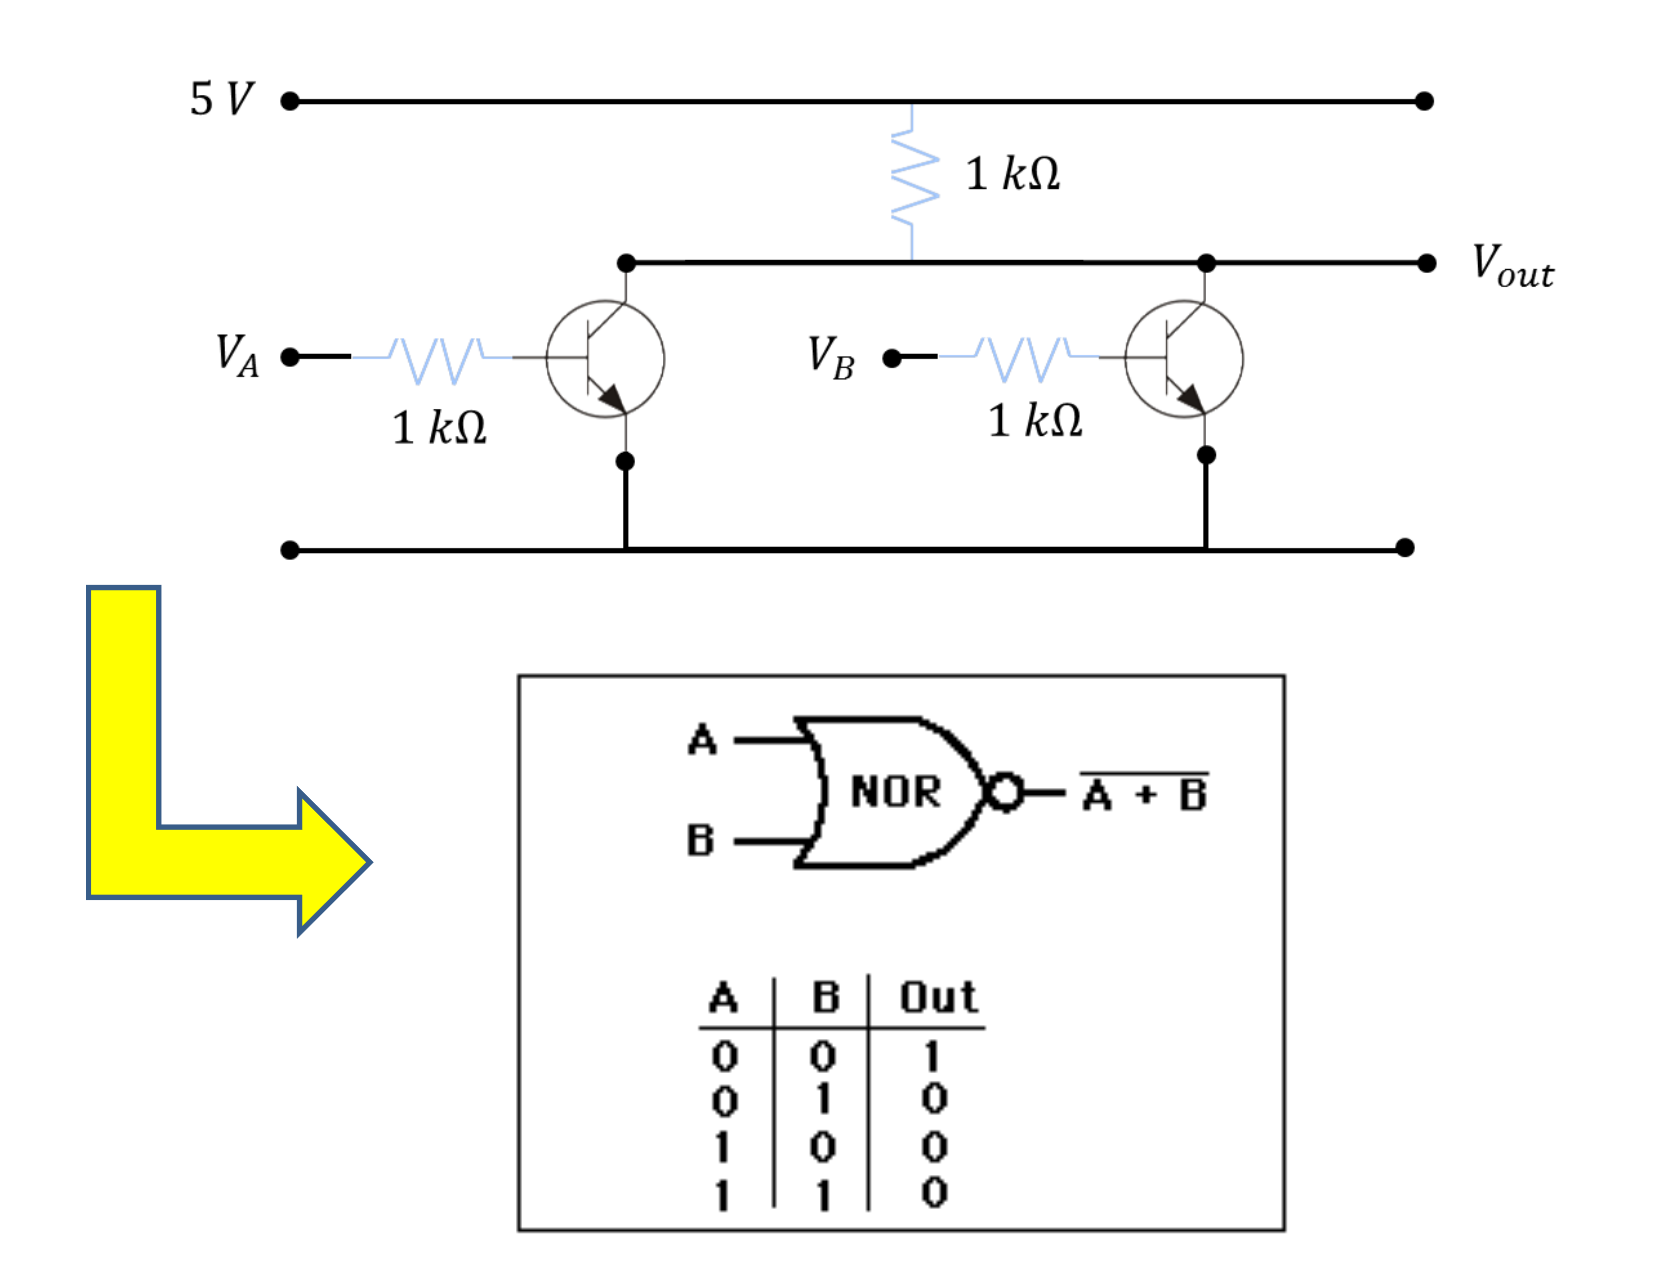
\includegraphics[width=\linewidth/2]{act4figure}
  \caption{The NOR gate circuit.}
  \label{fig:act4figure}
 \end{center}
\end{figure}

\begin{figure}[H]
 \begin{center}
  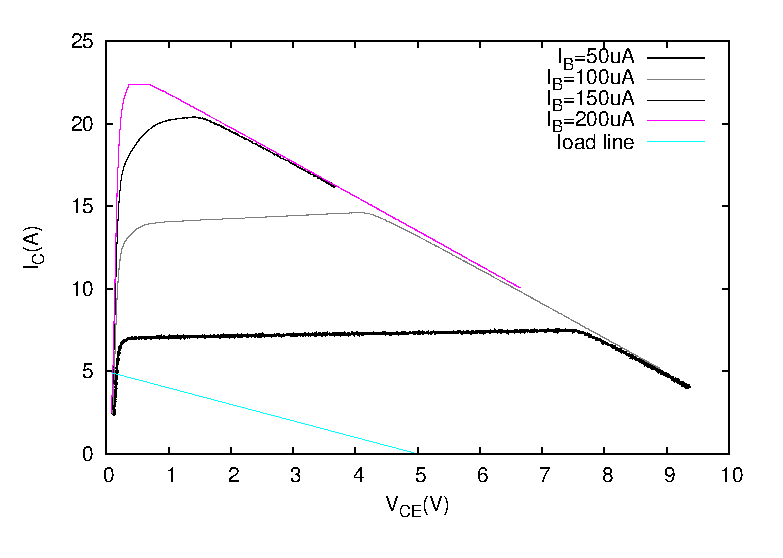
\includegraphics[width=\linewidth/1]{act4ll}
  \caption{The plot of $I_{\mathrm{c}}$ vs $V_{\mathrm{out}}$ with the load line ($V_{\mathrm{CC}}=5V$).}
  \label{fig:act4ll}
 \end{center}
\end{figure}

\end{document}
